\begin{textbox}{\href{https://compneuro.neuromatch.io/tutorials/W3D5_NetworkCausality/student/W3D5_Tutorial1.html}{Interventions (W3D5T1)}   }
\begin{subbox}{subbox}{Overview}
\scriptsize
Here we will describe causality, the tools we use to ask if and how a variable influences other variables. Causal questions are everywhere in neuroscience. How do neurons influence one another? How does a drug affect neurons? How does a stimulus affect behavior? We will talk about how we can answer questions of a causal kind. 
Causal questions are important all across neuroscience. For example, model fitting, machine learning, and dimensionality reduction, are often used to argue for or against causal models. For example, a regression may be used to argue that a brain region influences another brain region based on fMRI data. Today’s materials give us a better understanding of the problems that come with the approach. There are tight links between causality and Bayesian statistics where Bayesian techniques are used for the estimation of causality (see e.g. the work of Judea Pearl). Causality is often seen as the bedrock of science, today’s materials above all produce clarity about what it is.

Causality approaches are central across neuroscience. When we run experiments, we often randomly assign them to treatment groups vs control. Alternatively we stimulate animals at random points of time. These methods are all versions of randomized perturbations  and probably constitute a good part of all of neuroscience. We also use model fitting  frequently to drive arguments about how brains work. This is common for spike data, EEG data, imaging data etc. Lastly, we should be able to sometimes use instrumental variable techniques to estimate the effects of e.g. treatments with drugs. These materials are simultaneously at the heart of the field and are frequently ignored.

\end{subbox}
\end{textbox}
%%%%%%%%%%%%%%%%%%%%%%%%% 
%%%%%%%%%%%%%%%%%%%%%%%%%
\begin{textbox}{\href{https://compneuro.neuromatch.io/tutorials/W3D5_NetworkCausality/student/W3D5_Tutorial1.html}{Interventions (W3D5T1)}   }
\begin{subbox}{subbox}{Introduction}
\scriptsize
How do we know if a relationship is causal? What does that mean? And how can we estimate causal relationships within neural data?\\

The methods we'll learn today are very general and can be applied to all sorts of data, and in many circumstances.\\
Causal questions are everywhere!

\end{subbox}
\begin{subbox}{subbox}{Defining and estimating causality}
\scriptsize

Let's think carefully about the statement "\textbf{A causes B}". To be concrete, let's take two neurons. What does it mean to say that neuron $A$ causes neuron $B$ to fire?

The \textit{interventional} definition of causality says that:
\begin{eqnarray*}
(A \text{ causes } B) &\Leftrightarrow& ( \text{ If we force }A \\
& & \text { to be different, then }B\text{ changes})
\end{eqnarray*}

To determine if $A$ causes $B$ to fire, we can inject current into neuron $A$ and see what happens to $B$.\\

\textbf{A mathematical definition of causality:}\\
Over many trials, the average causal effect $\delta_{A\to B}$ of neuron $A$ upon neuron $B$ is the average change in neuron $B$'s activity when we set $A=1$ versus when we set $A=0$.


\begin{equation*}
\delta_{A\to B} = \mathbb{E}[B | A=1] -  \mathbb{E}[B | A=0] 
\end{equation*}


where $\mathbb{E}[B | A=1]$ is the expected value of B if A is 1 and  $\mathbb{E}[B | A=0]$ is the expected value of B if A is 0.

Note that this is an average effect. While one can get more sophisticated about conditional effects ($A$ only effects $B$ when it's not refractory, perhaps), we will only consider average effects today.


**Relation to a randomized controlled trial (RCT)**:
The logic we just described is the logic of a randomized control trial (RCT). If you randomly give 100 people a drug and 100 people a placebo, the effect is the difference in outcomes.

\end{subbox}
\begin{subbox}{subbox}{Randomized controlled trial for two neurons}
\scriptsize
Let's pretend we can perform a randomized controlled trial for two neurons. Our model will have neuron $A$ synapsing on Neuron $B$:

\begin{equation*}
B = A + \epsilon
\end{equation*}

where $A$ and $B$ represent the activities of the two neurons and $\epsilon$ is standard normal noise $\epsilon\sim\mathcal{N}(0,1)$.

To confirm if  $A$ is perturbed that $B$ changes.\\
We can calculate the a difference in means of `0.990719` (so very close to one)

\end{subbox}
\end{textbox}
%%%%%%%%%%%%%%%%%%%%%%%%% 
%%%%%%%%%%%%%%%%%%%%%%%%%
\begin{textbox}{\href{https://compneuro.neuromatch.io/tutorials/W3D5_NetworkCausality/student/W3D5_Tutorial1.html}{Interventions (W3D5T1)}   }
\begin{subbox}{subbox}{Simulating a system of neurons}
\scriptsize
Can we still estimate causal effects when the neurons are in big networks? This is the main question we will ask today. Let's first create our system, and the rest of today we will spend analyzing it.
Here we introduce a big causal system (interacting neurons) with understandable dynamical properties and how to simulate it.

Our system has N interconnected neurons that affect each other over time. Each neuron at time $t+1$ is a function of the activity of the other neurons from the previous time $t$. 

Neurons affect each other nonlinearly: each neuron's activity at time $t+1$ consists of a linearly weighted sum of all neural activities at time $t$, with added noise, passed through a nonlinearity:

\begin{equation*}
\vec{x}_{t+1} = \sigma(A\vec{x}_t + \epsilon_t),
\end{equation*}
\begin{itemize}
    \item 
 $\vec{x}_t$ is an $n$-dimensional vector representing our $n$-neuron system at timestep $t$
  \item $\sigma$ is a sigmoid nonlinearity
  \item $A$ is our $n \times n$ *causal ground truth connectivity matrix* (more on this later)
  \item $\epsilon_t$ is random noise: $\epsilon_t \sim N(\vec{0}, I_n)$
  \item $\vec{x}_0$ is initialized to $\vec{0}$
\end{itemize}

$A$ is a connectivity matrix, so the element $A_{ij}$ represents the causal effect of neuron $i$ on neuron $j$. In our system, neurons will receive connections from only 10\% of the whole population on average.

We will create the true connectivity matrix between 6 neurons and visualize it in two different ways: as a graph with directional edges between connected neurons and as an image of the connectivity matrix.

\textbf{Check your understanding}: do you understand how the left plot relates to the right plot below?
\begin{center}
    
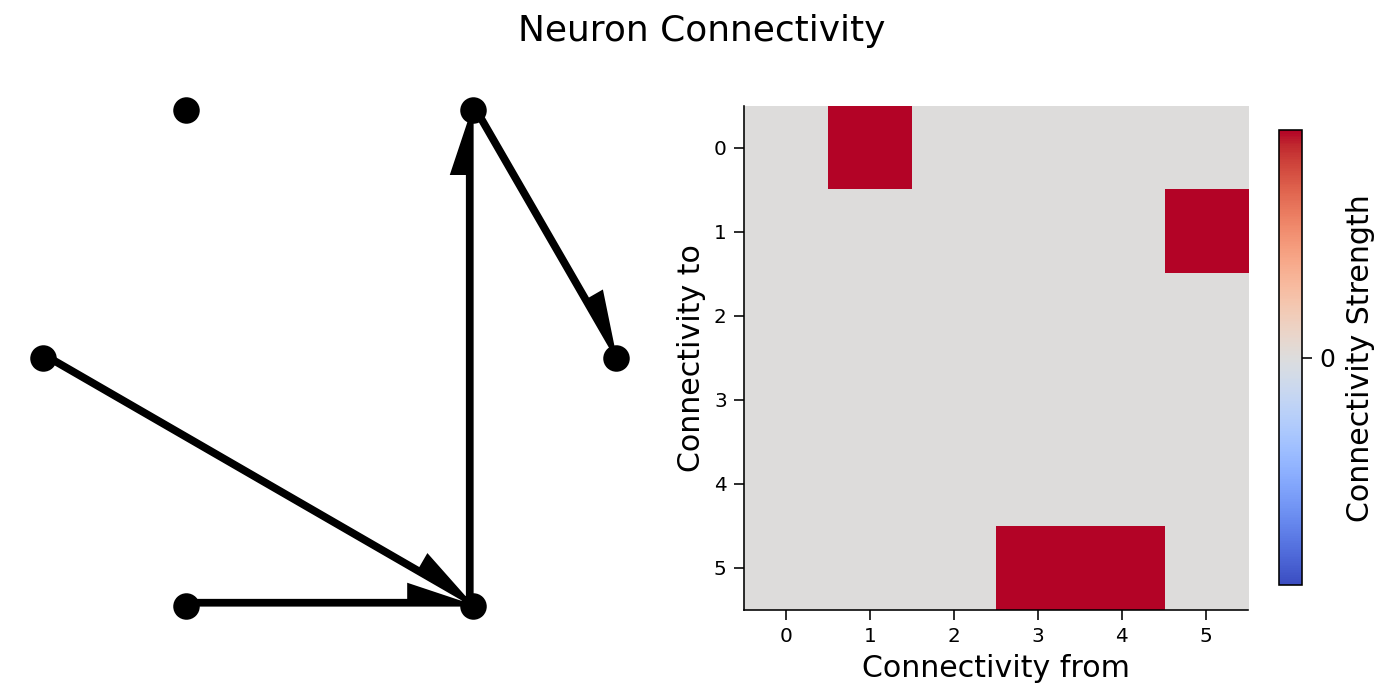
\includegraphics[scale=0.25]{Figures/NC/NC_Figure1.png}
\end{center}
\end{subbox}
\end{textbox}
%%%%%%%%%%%%%%%%%%%%%%%%% 
%%%%%%%%%%%%%%%%%%%%%%%%%
\begin{textbox}{\href{https://compneuro.neuromatch.io/tutorials/W3D5_NetworkCausality/student/W3D5_Tutorial1.html}{Interventions (W3D5T1)}   }
\begin{subbox}{subbox}{System simulation}
\scriptsize


To simulation a system of six neurons we using a sigmoid $\sigma$ function so that at every timestep the activity vector $x$ is updated according to: 
\begin{equation*}
\vec{x}_{t+1} = \sigma(A\vec{x}_t + \epsilon_t).
\end{equation*}
giving the plot:

\begin{center}
    
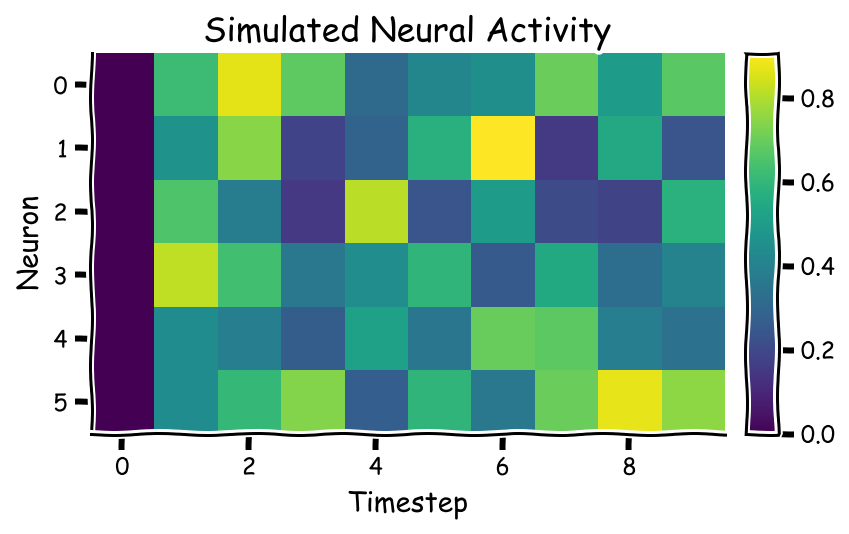
\includegraphics[scale=0.2]{Figures/NC/NC_Figure2.png}
\end{center}
\end{subbox}
\begin{subbox}{subbox}{Random perturbation in our system of neurons}
\scriptsize

We want to get the causal effect of each neuron upon each other neuron. The ground truth of the causal effects is the connectivity matrix $A$.

Remember that we would like to calculate:

\begin{eqnarray*}
\delta_{A\to B} &=& \mathbb{E}[B | A=1] -  \mathbb{E}[B | A=0] 
\end{eqnarray*}


We'll do this by randomly setting the system state to 0 or 1 and observing the outcome after one timestep. If we do this $N$ times, the effect of neuron $i$ upon neuron $j$ is:

\begin{eqnarray*}
\delta_{x^i\to x^j} &\approx& \frac1N \sum_{\substack{t=0, \ t \text{ even}}}^N[x_{t+1}^j | x^i_t=1] \\ & & - \frac1N \sum_{\substack{t=0, \ t \text{ even}}}^N[x_{t+1}^j | x^i_t=0]
\end{eqnarray*}

This is just the average difference of the activity of neuron $j$ in the two conditions.

We are going to calculate the above equation, but imagine it like \textit{intervening} in activity every other timestep.

\begin{center}
    
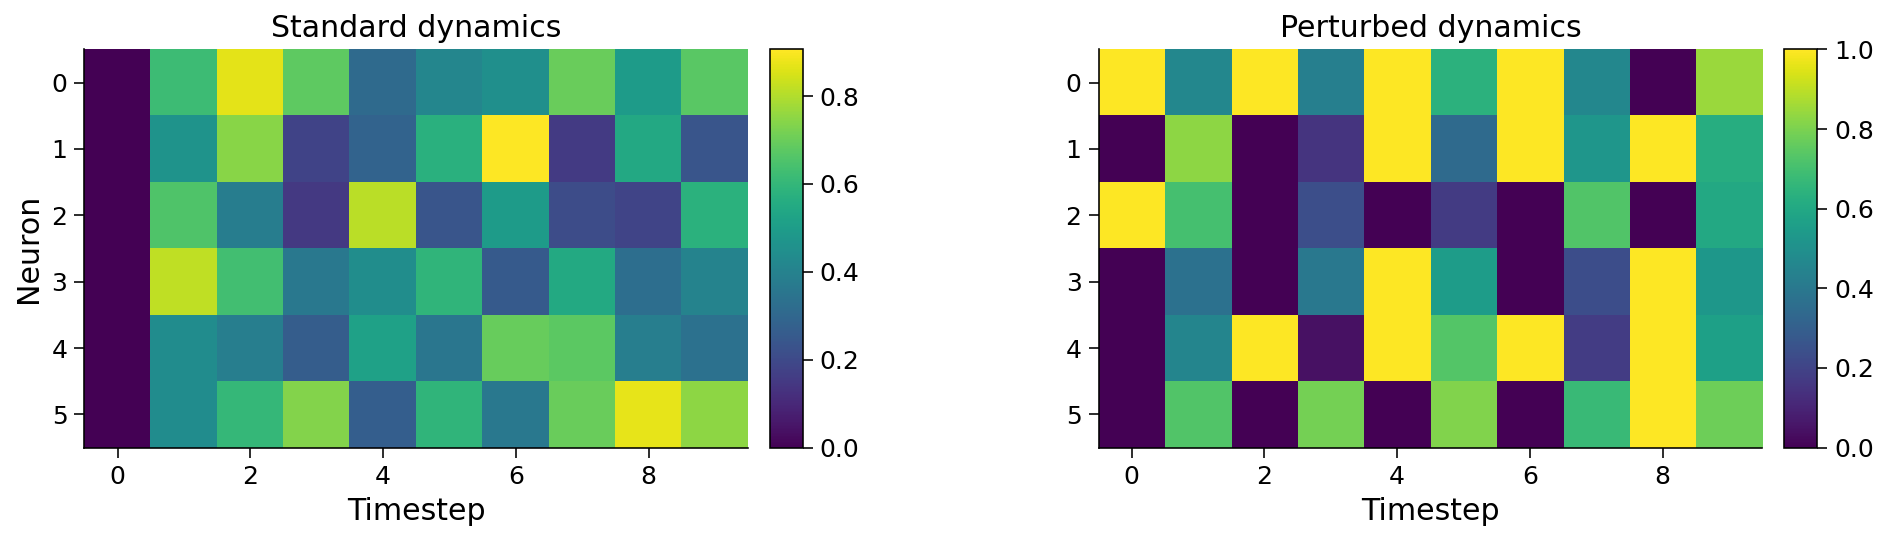
\includegraphics[scale=0.2]{Figures/NC/NC_Figure3.png}
\end{center}
\end{subbox}
\end{textbox}
%%%%%%%%%%%%%%%%%%%%%%%%% 
%%%%%%%%%%%%%%%%%%%%%%%%%
\begin{textbox}{\href{https://compneuro.neuromatch.io/tutorials/W3D5_NetworkCausality/student/W3D5_Tutorial1.html}{Interventions (W3D5T1)}   }

\begin{subbox}{subbox}{Recovering connectivity from perturbed dynamics}
\scriptsize

Recall that we perturbed every neuron at every other timestep. Despite perturbing every neuron, in this exercise we are concentrating on computing the causal effect of a single neuron (we will look at all neurons effects on all neurons next). We want to exclusively use the timesteps without perturbation for $x^j_{t+1}$ and the timesteps with perturbation for $x^j_{t}$ in the formulas above.

\begin{center}
    
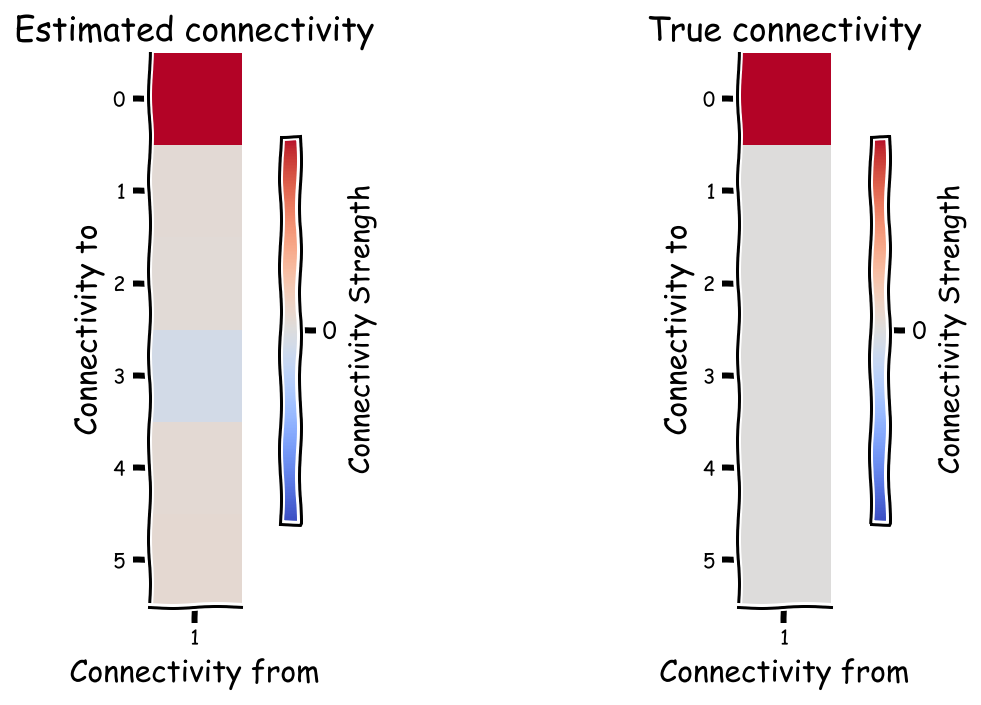
\includegraphics[scale=0.15]{Figures/NC/NC_Figure4.png}
\end{center}
We can quantify how close our estimated connectivity matrix is to our true connectivity matrix by correlating them. We should see almost perfect correlation between our estimates and the true connectivity - do we?

\textbf{Note on interpreting A}: Strictly speaking, $A$ is not the matrix of causal effects but rather the dynamics matrix. So why compare them like this? The answer is that $A$ and the effect matrix both are $0$ everywhere except where there is a directed connection. So they should have a correlation of $1$ if we estimate the effects correctly. (Their scales, however, are different. This is in part because the nonlinearity $\sigma$ squashes the values of $x$ to $[0,1]$.) 
\begin{center}
    
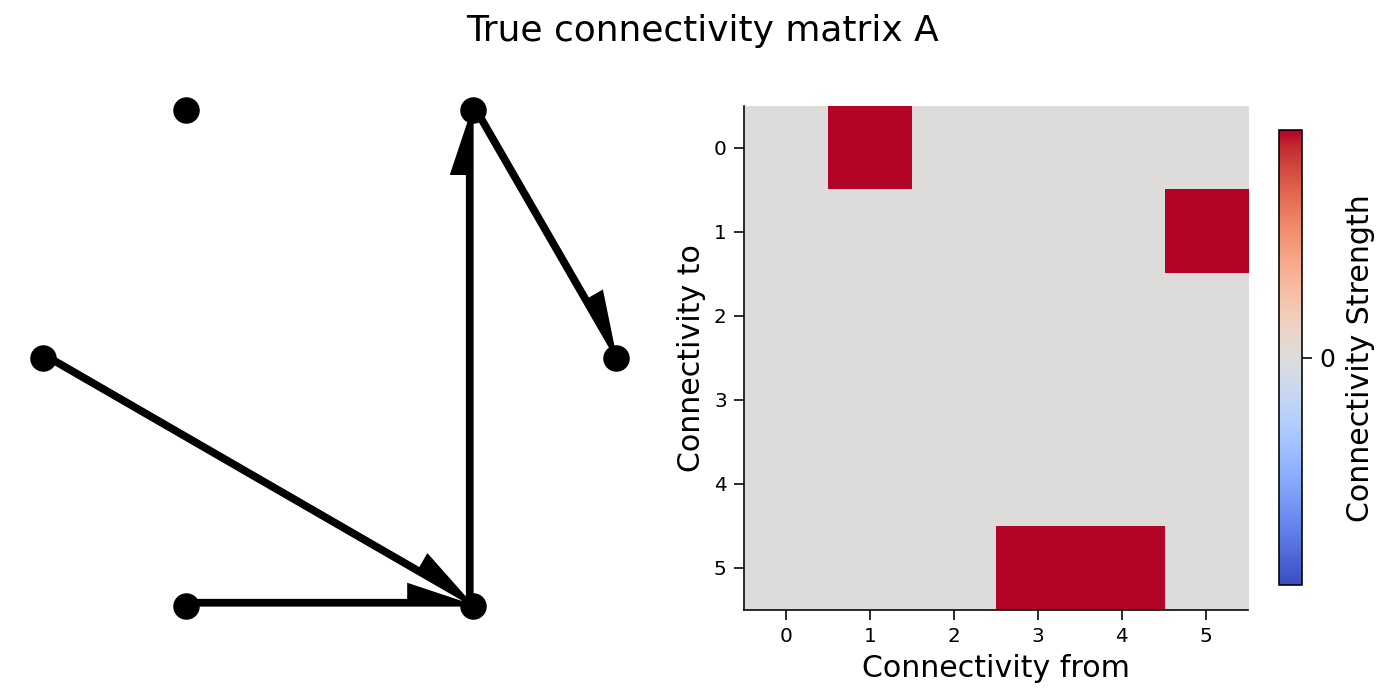
\includegraphics[scale=0.2]{Figures/NC/NC_Figure6.png}
\end{center}
\begin{center}
    
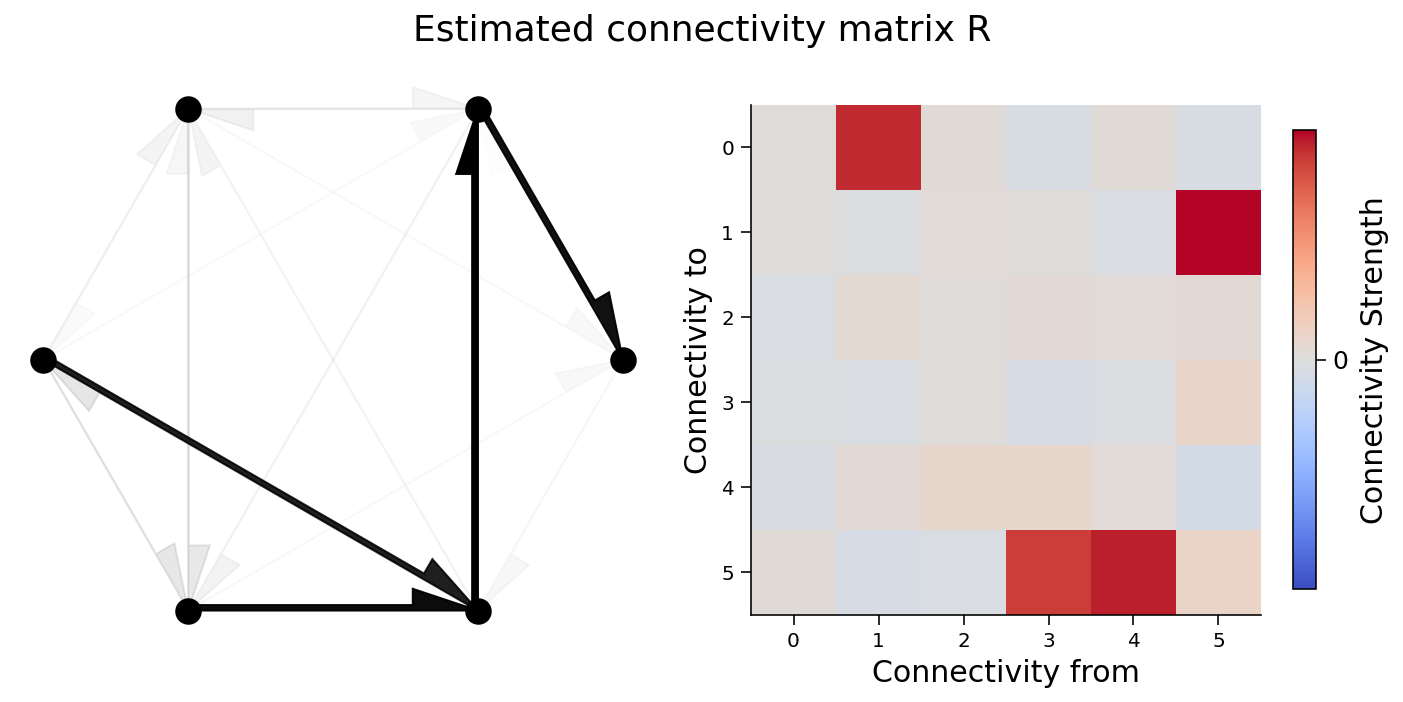
\includegraphics[scale=0.2]{Figures/NC/NC_Figure7.png}
\end{center}
We can again calculate the correlation coefficient between the elements of the two matrices.
If it is almost 1 we have done a good job recovering the true causality of the system!

\end{subbox}
\end{textbox}
\newpage
%%%%%%%%%%%%%%%%%%%%%%%%% 
%%%%%%%%%%%%%%%%%%%%%%%%%
%%% TUTORIAL 2
%%%%%%%%%%%%%%%%%%%%%%%%% 
%%%%%%%%%%%%%%%%%%%%%%%%%
\begin{textbox}{\href{https://compneuro.neuromatch.io/tutorials/W3D5_NetworkCausality/student/W3D5_Tutorial2.html}{Correlations (W3D5T2)}   }

\begin{subbox}{subbox}{Recovering connectivity from perturbed dynamics}
\scriptsize


Here, we implemented and explored the dynamical system of neurons we will be working with throughout all of the tutorials today. We also learned about the "gold standard" of measuring causal effects through random perturbations. As random perturbations are often not possible, we will now turn to alternative methods to attempt to measure causality. We will:

\begin{itemize}
    \item  Learn how to estimate connectivity from observations assuming \textbf{correlations approximate causation}
\item Show that this only works when the network is small
\end{itemize}


Often, we can't force neural activities or brain areas to be on or off. We just have to observe. Maybe we can get the correlation between two nodes -- is that good enough? The question we ask here is \textbf{when is correlation a "good enough" substitute for causation?}

The answer is not "never", actually, but "sometimes".
\end{subbox}
\begin{subbox}{subbox}{Try to approximate causation with correlation}
\scriptsize



In small systems, correlation can look like causation. Let's attempt to recover the true connectivity matrix (A) just by correlating the neural state at each timestep with the previous state: $$C=\vec{x_t}{\vec{x_{t+1}}^\top}.$$ 

To calculate the connectivity matrix of a single neuron by calculating the correlation coefficients with every other neuron which correlate two vectors: 1) the activity of a selected neuron at time $t$ 2) The activity of all other neurons at time $t+1$.

The matrix answer is the same as the summation form.
Furthermore the estimated vs true connectivity look the same using the matrix calculation.

\begin{center}
    
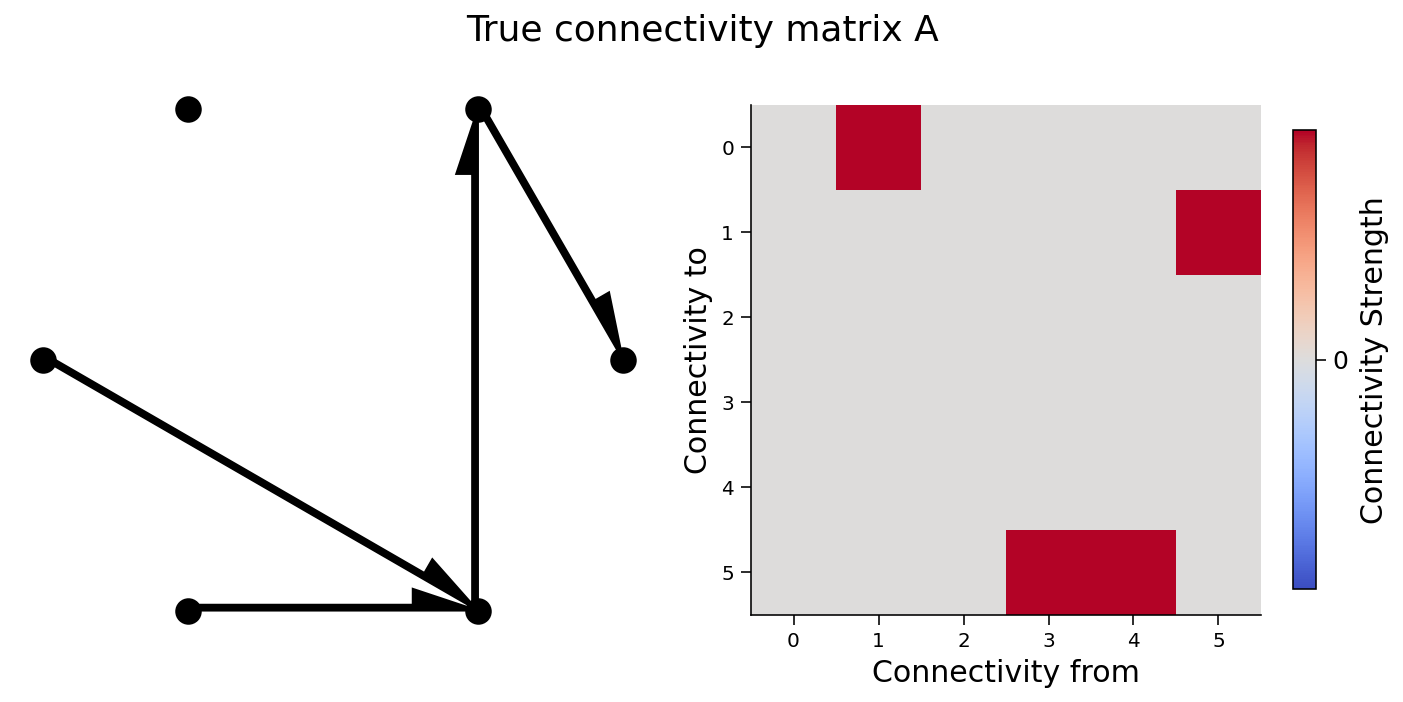
\includegraphics[scale=0.2]{Figures/NC/NC_Figure9.png}
    
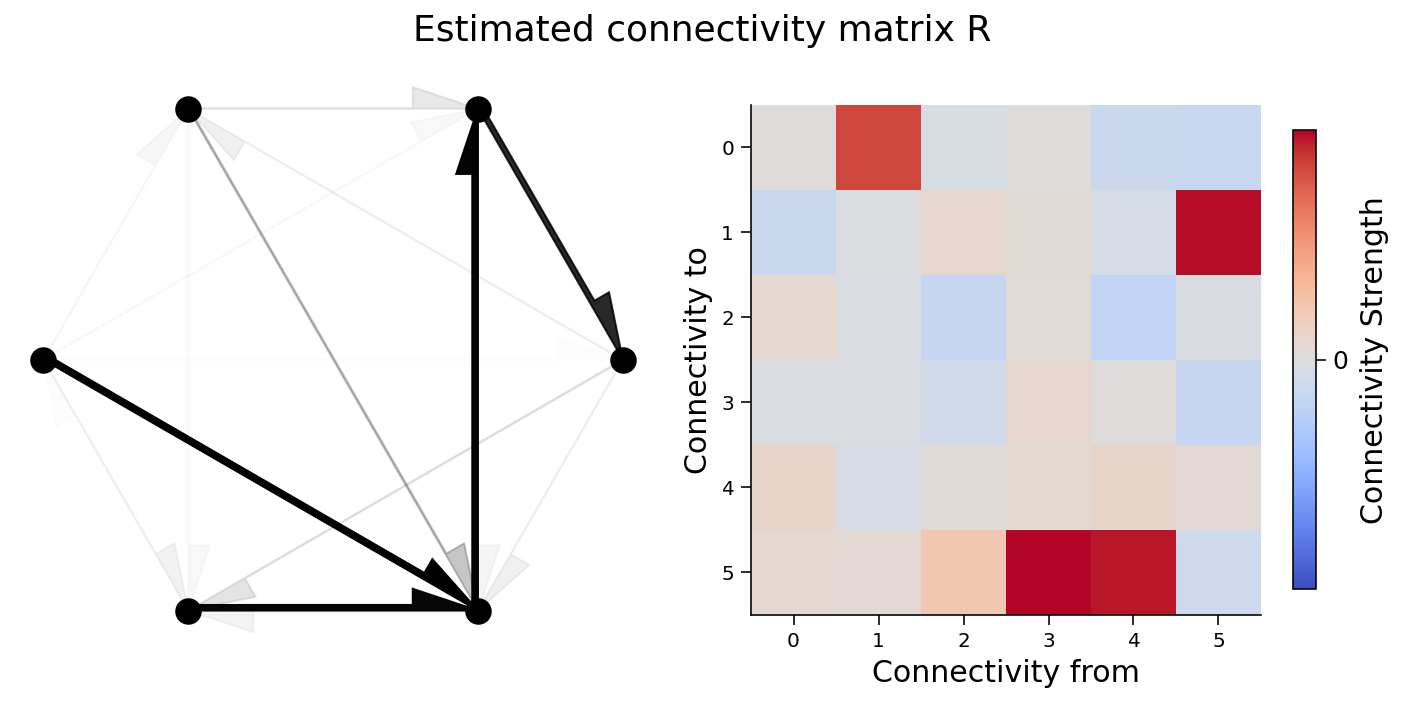
\includegraphics[scale=0.2]{Figures/NC/NC_Figure10.png}
\end{center}
\end{subbox}
\end{textbox}
%%%%%%%%%%%%%%%%%%%%%%%%%
%%%%%%%%%%%%%%%%%%%%%%%%%
\begin{textbox}{\href{https://compneuro.neuromatch.io/tutorials/W3D5_NetworkCausality/student/W3D5_Tutorial2.html}{Correlations (W3D5T2)}   }

\begin{subbox}{subbox}{Large systems}
\scriptsize

As our system becomes more complex however, correlation fails to capture causality.
Let's jump to a much bigger system. Instead of 6 neurons, we will now use 100 neurons. How does the estimation quality of the connectivity matrix change? 
\begin{center}

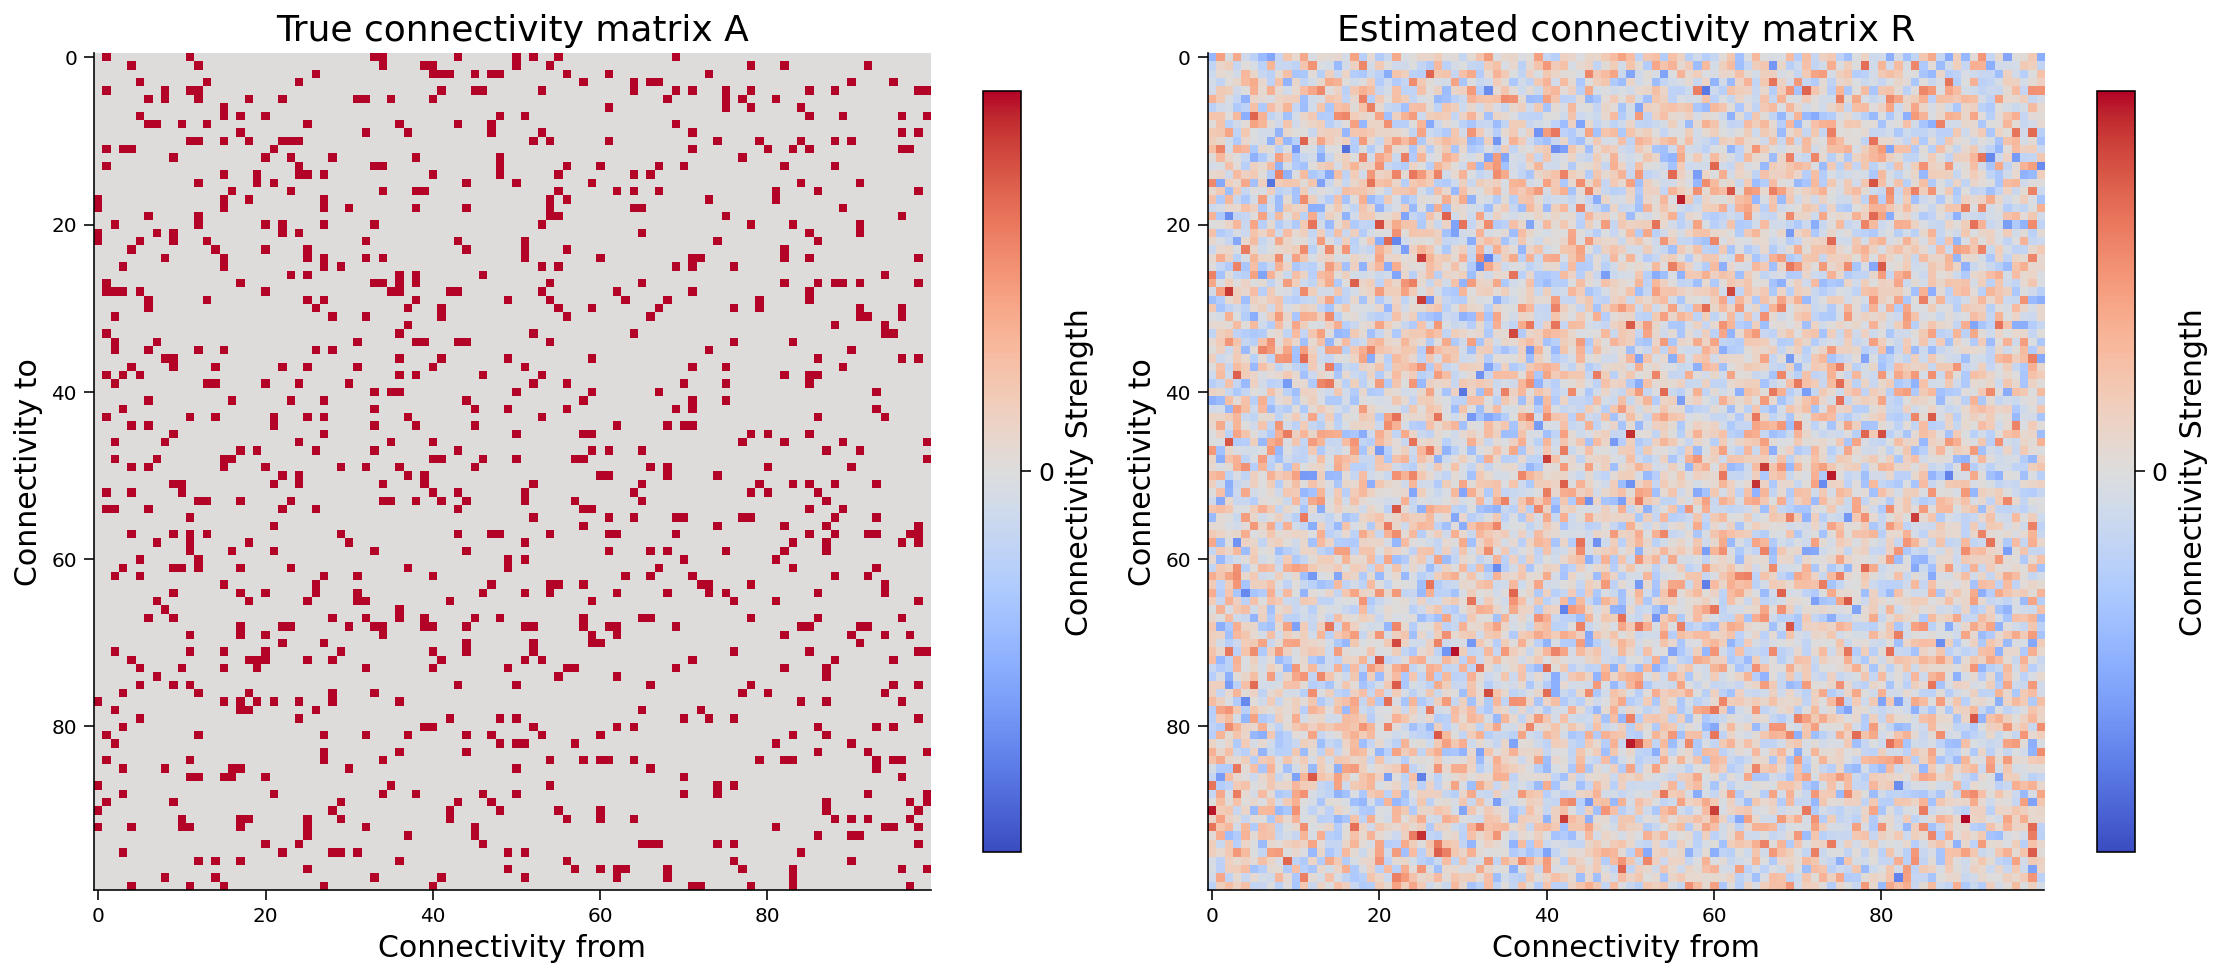
\includegraphics[scale=0.18]{Figures/NC/NC_Figure11.png}
\end{center}
\end{subbox}

\begin{subbox}{subbox}{Correlation as a function of network size}
\scriptsize
\begin{center}

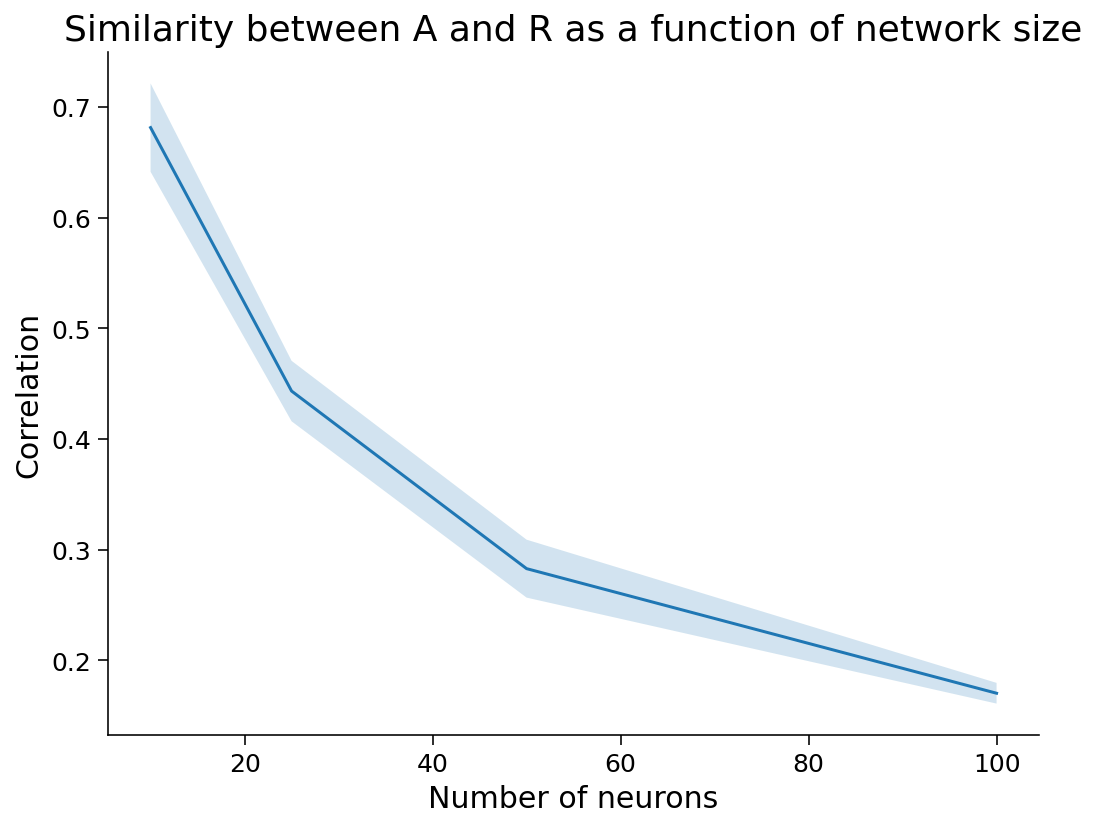
\includegraphics[scale=0.15]{Figures/NC/NC_Figure13.png}
\end{center}
\end{subbox}
\begin{subbox}{subbox}{Connectivity estimation as a function of the sparsity of $A$}
\scriptsize

You may rightly wonder if correlation only fails for large systems for certain types of $A$. Does connectivity estimation get better or worse with less sparsity?

\begin{center}

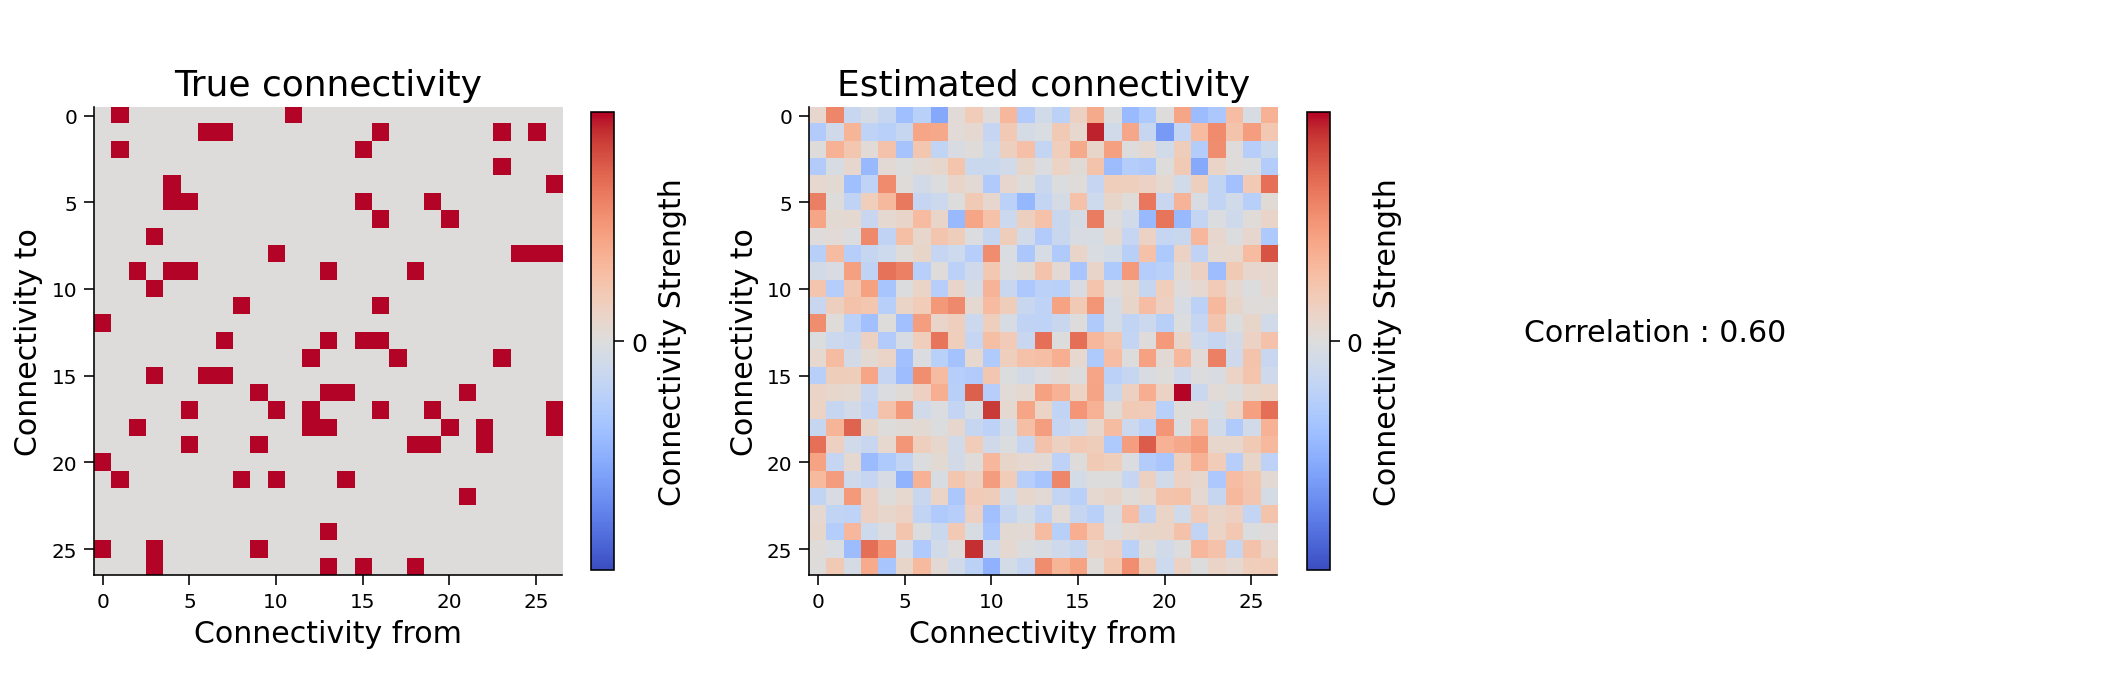
\includegraphics[scale=0.15]{Figures/NC/NC_Figure12.png}
\end{center}
\end{subbox}

\begin{subbox}{subbox}{Summary}
\scriptsize


Now for the takeaway. We know that for large systems correlation $\not=$ causation. But what about when we coarsely sample the large system? Do we get better at estimating the effective causal interaction between groups (=average of weights) from the correlation between the groups?

From our simulation above, the answer appears to be no: as the number of neurons per group increases, we don't see any significant increase in our ability to estimate the causal interaction between groups.

\end{subbox}
\end{textbox}
\newpage
%%%%%%%%%%%%%%%%%%%%%%%%%
%%%%%%%%%%%%%%%%%%%%%%%%%
%%%% TUTORIAL 3
%%%%%%%%%%%%%%%%%%%%%%%%%
%%%%%%%%%%%%%%%%%%%%%%%%%
\begin{textbox}{\href{https://compneuro.neuromatch.io/tutorials/W3D5_NetworkCausality/student/W3D5_Tutorial3.html}{Simultaneous fitting/regression (W3D5T3)}   }

\begin{subbox}{subbox}{Objectives}
\scriptsize


We have explored correlation as an approximation for causation and learned that correlation $\neq$ causation for larger networks. However, computing correlations is a rather simple approach, and you may be wondering: will more sophisticated techniques allow us to better estimate causality? Can't we control things? 

Here we'll use some common advanced (but controversial) methods that estimate causality from observational data. These methods rely on fitting a function to our data directly, instead of trying to use perturbations or correlations. Since we have the full closed-form equation of our system, we can try these methods and see how well they work in estimating causal connectivity when there are no perturbations. Specifically, we will:

\begin{itemize}
    \item  Learn about more advanced (but also controversial) techniques for estimating causality
    \item conditional probabilities (\textbf{regression})
\item Explore limitations and failure modes
    \item  understand the problem of \textbf{omitted variable bias}
\end{itemize}

\end{subbox}

\begin{subbox}{subbox}{Regression approach}
\scriptsize

You may be familiar with the idea that correlation only implies causation when there are no hidden \textit{confounders}. This aligns with our intuition that correlation only implies causality when no alternative variables could explain away a correlation.

\textbf{A confounding example}:\\
Suppose you observe that people who sleep more do better in school. It's a nice correlation. But what else could explain it? Maybe people who sleep more are richer, don't work a second job, and have time to actually do homework. If you want to ask if sleep \textit{causes} better grades, and want to answer that with correlations, you have to control for all possible confounds.\\

A confound is any variable that affects both the outcome and your original covariate. In our example, confounds are things that affect both sleep and grades. 

\textbf{Controlling for a confound}: 
Confounds can be controlled for by adding them as covariates in a regression. But for your coefficients to be causal effects, you need three things:
 \begin{enumerate}
     \item 
 All confounds are included as covariates
\item  Your regression assumes the same mathematical form of how covariates relate to outcomes (linear, GLM, etc.)
\item  No covariates are caused *by* both the treatment (original variable) and the outcome. These are \href{https://en.wikipedia.org/wiki/Collider_(statistics)}{colliders}; we won't introduce it today (but Google it on your own time! Colliders are very counterintuitive.)
 \end{enumerate}

In the real world it is very hard to guarantee these conditions are met. In the brain it's even harder (as we can't measure all neurons). Luckily today we simulated the system ourselves.

\end{subbox}
\end{textbox}
%%%%%%%%%%%%%%%%%%%%%%%%%
%%%%%%%%%%%%%%%%%%%%%%%%%
\begin{textbox}{\href{https://compneuro.neuromatch.io/tutorials/W3D5_NetworkCausality/student/W3D5_Tutorial3.html}{Simultaneous fitting/regression (W3D5T3)}   }

\begin{subbox}{subbox}{Fitting a General Linear Model (GLM)}
\scriptsize
We will use a regression approach to estimate the causal influence of all neurons to neuron #1. Specifically, we will use linear regression to determine the $A$ in:
\begin{equation}
\sigma^{-1}(\vec{x}_{t+1}) = A\vec{x}_t + \epsilon_t ,
\end{equation}
where $\sigma^{-1}$ is the inverse sigmoid transformation, also sometimes referred to as the \textbf{logit} transformation: $\sigma^{-1}(x) = \log(\frac{x}{1-x})$.

Let $W$ be the $\vec{x}_t$ values, up to the second-to-last timestep $T-1$:
\begin{equation}
W = 
\begin{bmatrix}
\mid & \mid & ... & \mid \\ 
\vec{x}_0  & \vec{x}_1  & ... & \vec{x}_{T-1}  \\ 
\mid & \mid & ... & \mid
\end{bmatrix}_{n \times (T-1)}
\end{equation}

Let $Y$ be the $\vec{x}_{t+1}$ values for a selected neuron, indexed by $i$, starting from the second timestep up to the last timestep $T$:

\begin{equation}
Y = 
\begin{bmatrix}
x_{i,1}  & x_{i,2}  & ... & x_{i, T}  \\ 
\end{bmatrix}_{1 \times (T-1)}
\end{equation}

You then fit the following model:

\begin{equation}
\sigma^{-1}(Y^T) = W^TV
\end{equation}

where $V$ is the $n \times 1$ coefficient matrix of this regression, which will be the estimated connectivity matrix between the selected neuron and the rest of the neurons.


We can see that multiple regression is better than simple correlation for estimating connectivity.


\end{subbox}

\end{textbox}
%%%%%%%%%%%%%%%%%%%%%%%%%
%%%%%%%%%%%%%%%%%%%%%%%%%
\begin{textbox}{\href{https://compneuro.neuromatch.io/tutorials/W3D5_NetworkCausality/student/W3D5_Tutorial3.html}{Simultaneous fitting/regression (W3D5T3)}   }

\begin{subbox}{subbox}{Partially Observed Systems}
\scriptsize
If we are unable to observe the entire system, \textbf{omitted variable bias} becomes a problem. If we don't have access to all the neurons, and so therefore can't control them, can we still estimate the causal effect accurately?

We first visualize different subsets of the connectivity matrix when we observe 75\% of the neurons vs 25\%.

Recall the meaning of entries in our connectivity matrix: $A[i,j] = 1$ means a connectivity from neuron $i$ to neuron $j$ with strength $1$.
\begin{center}
    
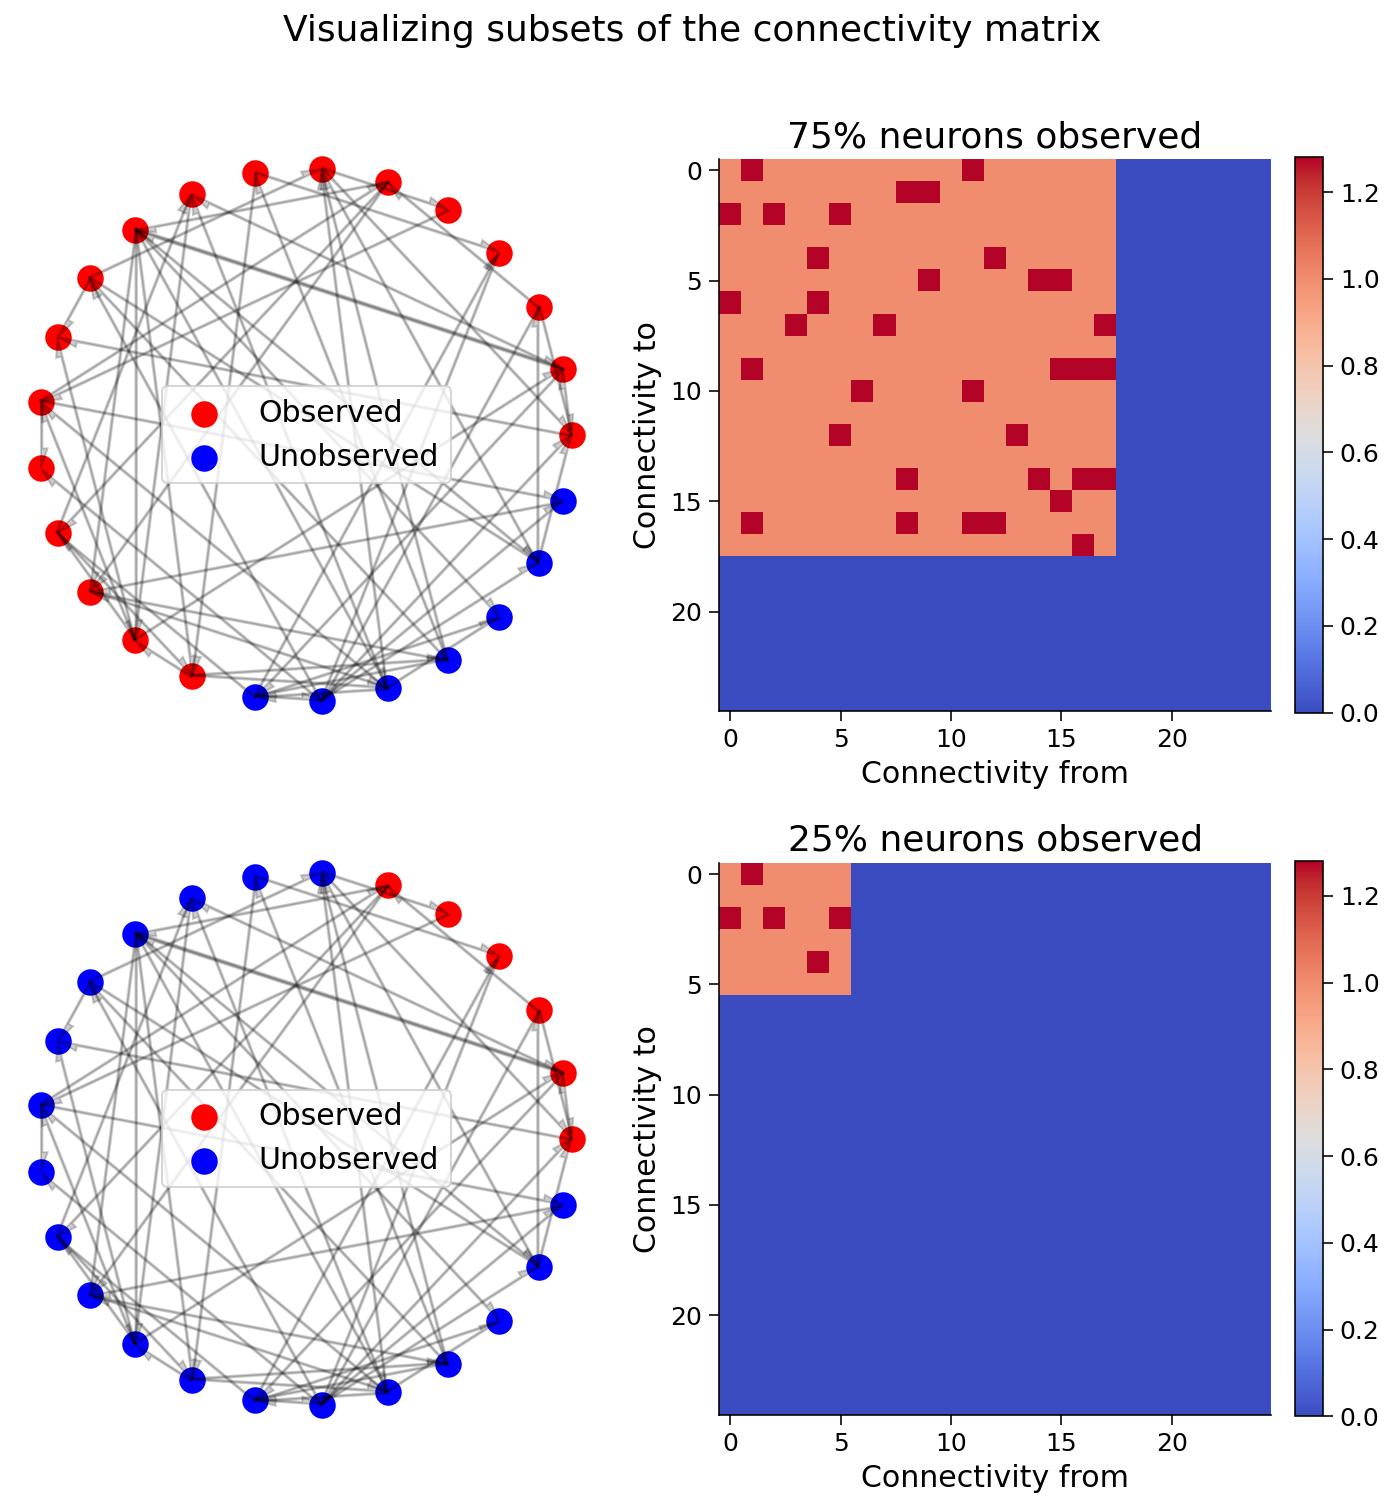
\includegraphics[scale=0.24]{Figures/NC/NC_Figure15.png}

\end{center}

Next, we will inspect a plot of the correlation between true and estimated connectivity matrices vs the percent of neurons observed over multiple trials.
What is the relationship that you see between performance and the number of neurons observed?

\begin{center}
    
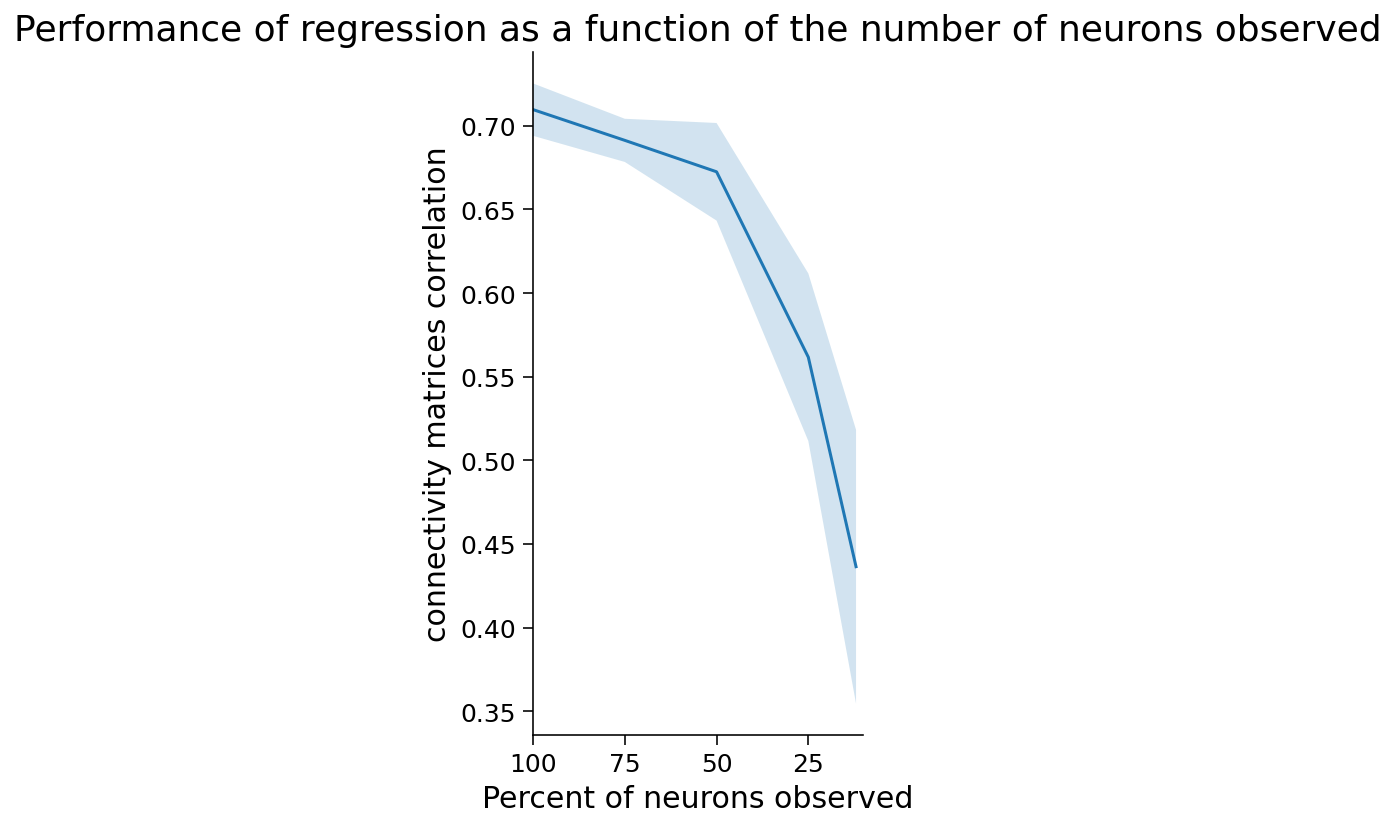
\includegraphics[scale=0.25]{Figures/NC/NC_Figure17.png}

\end{center}
\end{subbox}

\end{textbox}
\newpage
%%%%%%%%%%%%%%%%%%%%%%%%%
%%%%%%%%%%%%%%%%%%%%%%%%%
%%%% TUTORIAL 4
%%%%%%%%%%%%%%%%%%%%%%%%%
%%%%%%%%%%%%%%%%%%%%%%%%%
\begin{textbox}{\href{https://compneuro.neuromatch.io/tutorials/W3D5_NetworkCausality/student/W3D5_Tutorial4.html}{Instrumental Variables (W3D5T4)}   }

\begin{subbox}{subbox}{Objectives}
\scriptsize


We have seen that even more sophisticated techniques such as simultaneous fitting fail to capture causality in the presence of omitted variable bias. So what techniques are there for us to obtain valid causal measurements when we can't perturb the system? Here we will:
\begin{itemize}
    \item 
 learn about \textbf{instrumental variables}, a method that does not require experimental data for valid causal analysis
\item  explore benefits of instrumental variable analysis and limitations
 \item  addresses \textbf{omitted variable bias} seen in regression
   \item  less efficient in terms of sample size than other techniques
 \item  requires a particular form of randomness in the system in order for causal effects to be identified
    \end{itemize}

\end{subbox}

\begin{subbox}{subbox}{Instrumental Variables}
\scriptsize

If there is randomness naturally occurring in the system \textit{that we can observe}, this in effect becomes the perturbations we can use to recover causal effects. This is called an \textbf{instrumental variable}. At high level, an instrumental variable must
\begin{enumerate}
    
\item Be observable
\item  Affect a covariate you care about
\item  \textbf{Not} affect the outcome, except through the covariate
\end{enumerate}

It's rare to find these things in the wild, but when you do it's very powerful.
\begin{center}
    
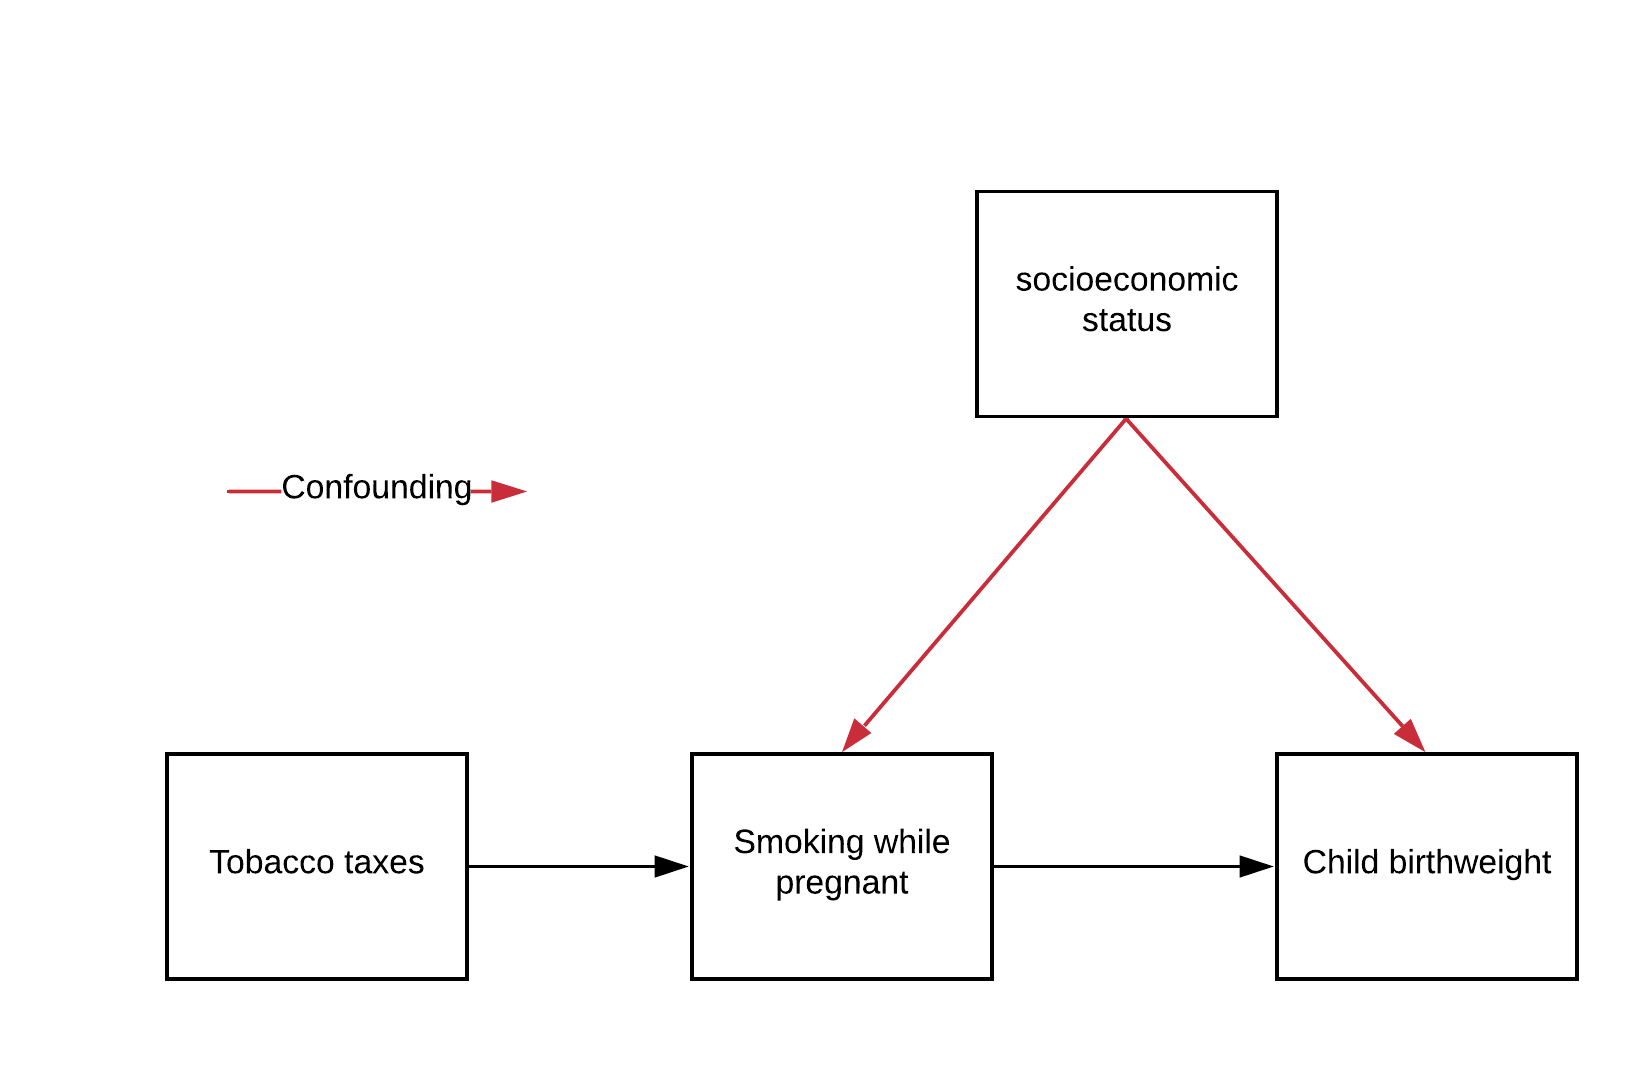
\includegraphics[scale=0.15]{Figures/NC/NC_Figure18.png}

\end{center}
\end{subbox}
\end{textbox}
%%%%%%%%%%%%%%%%%%%%%%%%%%%%%%%%%%
%%%%%%%%%%%%%%%%%%%%%%%%%
\begin{textbox}{\href{https://compneuro.neuromatch.io/tutorials/W3D5_NetworkCausality/student/W3D5_Tutorial4.html}{Instrumental Variables (W3D5T4)}   }
\begin{subbox}{subbox}{A non-neuro example of an Instrumental Variables (IV)}
\scriptsize

A classic example is estimating the effect of smoking cigarettes while pregnant on the birth weight of the infant. There is a (negative) correlation, but is it causal? Unfortunately many confounds affect both birth weight and smoking. Wealth is a big one. Instead of controlling everything imaginable, one can find an IV. Here the instrumental variable is \textbf{state taxes on tobacco}. These

\begin{enumerate}
    \item    Are observable
    \item   Affect tobacco consumption
    \item   Don't affect birth weight except through tobacco
\end{enumerate}

By using the power of IV techniques, you can determine the causal effect without exhaustively controlling for everything.

Let's represent our tobacco example above with the following notation:
\begin{itemize}
    \item 
 $Z_{\text{taxes}}$: our tobacco tax \textit{instrument}, which only affects an individual's tendency to smoke while pregnant within our system
\item $T_{\text{smoking}}$: number of cigarettes smoked per day while pregnant, our "treatment" if this were a randomized trial
\item $C_{\text{SES}}$: socioeconomic status (higher means wealthier), a \textit{confounder} if it is not observed
\item
$Y_{\text{birthweight}}$: child birthweight in grams, our outcome of interest
\end{itemize}

Let's suppose we have the following function for our system:
$$Y_{\text{birthweight}} = 3000 + C_{\text{SES}} - 2T_{\text{smoking}},$$
with the additional fact that $C_{\text{SES}}$ is negatively correlated with $T_{\text{smoking}}$. 

The causal effect we wish to estimate is the coefficient $-2$ for $T_{\text{smoking}}$, which means that if a mother smokes one additional cigarette per day while pregnant her baby will be 2 grams lighter at birth. We've provided a covariance matrix with the desired structure in the code cell below, so please run it to look at the correlations between our variables.\\
Correlation between SES status and cigarettes: -0.483\\
Correlation between SES status and birth weight: 0.740\\
We see what is exactly represented in our graph above: $C_{\text{SES}}$ is correlated with both $T_{\text{smoking}}$ and $Y_{\text{birthweight}}$, so $C_{\text{SES}}$ is a potential confounder if not included in our analysis. Let's say that it is difficult to observe and quantify $C_{\text{SES}}$, so we do not have it available to regress against. This is another example of the \textbf{omitted variable bias}.\\
What about $Z_{\text{taxes}}$?\\
Correlation between taxes and cigarettes: 0.519\\
Correlation between taxes and SES status: 0.009\\
Perfect! We see that $Z_{\text{taxes}}$ is correlated with $T_{\text{smoking}}$ (#2) but is uncorrelated with $C_{\text{SES}}$ (#3).  $Z_\text{taxes}$ is also observable (#1), so we've satisfied our three criteria for an instrument:
\begin{enumerate}
    \item 
   $Z_\text{taxes}$ is observable
\item    $Z_\text{taxes}$ affects $T_{\text{smoking}}$
\item    $Z_\text{taxes}$ doesn't affect
\end{enumerate}
$Y_{\text{birthweight}}$ except through $T_{\text{smoking}}$ (ie $Z_\text{taxes}$ doesn't affect or is affected by $C_\text{SES}$)

\end{subbox}
\end{textbox}
%%%%%%%%%%%%%%%%%%%%%%%%%
%%%%%%%%%%%%%%%%%%%%%%%%%
\begin{textbox}{\href{https://compneuro.neuromatch.io/tutorials/W3D5_NetworkCausality/student/W3D5_Tutorial4.html}{Instrumental Variables (W3D5T4)}   }
\begin{subbox}{subbox}{ How IV works, at high level
}
\scriptsize
The easiest way to imagine IV is that the instrument is \textbf{an observable source of "randomness"} that affects the treatment. In this way it's similar to the interventions we talked about in Tutorial 1.

But how do you actually use the instrument? The key is that we need to extract \textbf{the component of the treatment that is due only to the effect of the instrument}. We will call this component $\hat{T}$.
$$
\hat{T}\leftarrow \text{The unconfounded component of }T
$$
Getting $\hat{T}$ is fairly simple. It is simply the predicted value of $T$ found in a regression that has only the instrument $Z$ as input.

Once we have the unconfounded component in hand, getting the causal effect is as easy as regressing the outcome on $\hat{T}$.

\end{subbox}
\begin{subbox}{subbox}{ IV estimation using two-stage least squares
}
\scriptsize
The fundamental technique for instrumental variable estimation is \textbf{two-stage least squares}. 

We run two regressions:
\begin{enumerate}
    \item 
 The first stage gets  $\hat{T}_{\text{smoking}}$ by regressing $T_{\text{smoking}}$ on $Z_\text{taxes}$, fitting the parameter $\hat{\alpha}$:

\begin{equation}
\hat{T}_{\text{smoking}} = \hat{\alpha} Z_\text{taxes}
\end{equation}

\item The second stage then regresses $Y_{\text{birthweight}}$ on $\hat{T}_{\text{smoking}}$ to obtain an estimate $\hat{\beta}$ of the causal effect:
\end{enumerate}

\begin{equation}
\hat{Y}_{\text{birthweight}} = \hat{\beta} \hat{T}_{\text{smoking}} 
\end{equation}

The first stage estimates the \textbf{unconfounded component} of $T_{\text{smoking}}$ (ie, unaffected by the confounder $C_{\text{SES}}$), as we discussed above. 

Then, the second stage uses this unconfounded component $\hat{T}_{\text{smoking}}$ to estimate the effect of smoking on $\hat{Y}_{\text{birthweight}}$. 

\textbf{Compute regression stage 1}\\

Let's run the regression of $T_{\text{smoking}}$ on $Z_\text{taxes}$ to compute $\hat{T}_{\text{smoking}}$. We will then check whether our estimate is still confounded with $C_{\text{SES}}$ by comparing the correlation of $C_{\text{SES}}$  with $T_{\text{smoking}}$ vs $\hat{T}_{\text{smoking}}$.\\
The result of the correlation between $T$ and $C$ of `-0.483` and between $\hat{T}$ and $C$ of `0.009`.\\

\textbf{Least squares regression stage 2}\\
Now let's implement the second stage! We will again use a linear regression model with an intercept. We will obtain the estimated causal effect of the number of cigarettes ($T$) on birth weight ($Y$).\\

The result of estimated causal effect of `-1.984`, This is quite close to the true causal effect of $-2$!

\end{subbox}
\end{textbox}
%%%%%%%%%%%%%%%%%%%%%%%%%
%%%%%%%%%%%%%%%%%%%%%%%%%
\begin{textbox}{\href{https://compneuro.neuromatch.io/tutorials/W3D5_NetworkCausality/student/W3D5_Tutorial4.html}{Instrumental Variables (W3D5T4)}   }
\begin{subbox}{subbox}{ IVs in our simulated neural system
}
\scriptsize
Now, say we have the neural system we have been simulating, except with an additional variable $\vec{z}$. This will be our instrumental variable. 

We treat $\vec{z}$ as a source of noise in the dynamics of our neurons:

\begin{equation}
\vec{x}_{t+1} = \sigma(A\vec{x}_t + \eta \vec{z}_{t+1} + \epsilon_t)
\end{equation}

where $\eta$ is what we'll call the "strength" of our IV, and $\vec{z}_t$ is a random binary variable, $\vec{z}_t \sim Bernoulli(0.5)$

Remember that for each neuron $i$, we are trying to figure out whether $i$ is connected to (causally affects) the other neurons in our system *at the next time step*. So for timestep $t$, we want to determine whether $\vec{x}_{i,t}$ affects all the other neurons at $\vec{x}_{t+1}$. For a given neuron $i$, $\vec{z}_{i,t}$ satisfies the 3 criteria for a valid instrument. \\

\textbf{What could $z$ be, biologically?}\\

Imagine $z$ to be some injected current through an \textit{in vivo} patch clamp. It affects each neuron individually, and only affects dynamics through that neuron.

The cool thing about IV is that you don't have to control $z$ yourself - it can be observed. So if you mess up your wiring and accidentally connect the injected voltage to an AM radio, no worries. As long as you can observe the signal the method will work.
\begin{center}
    
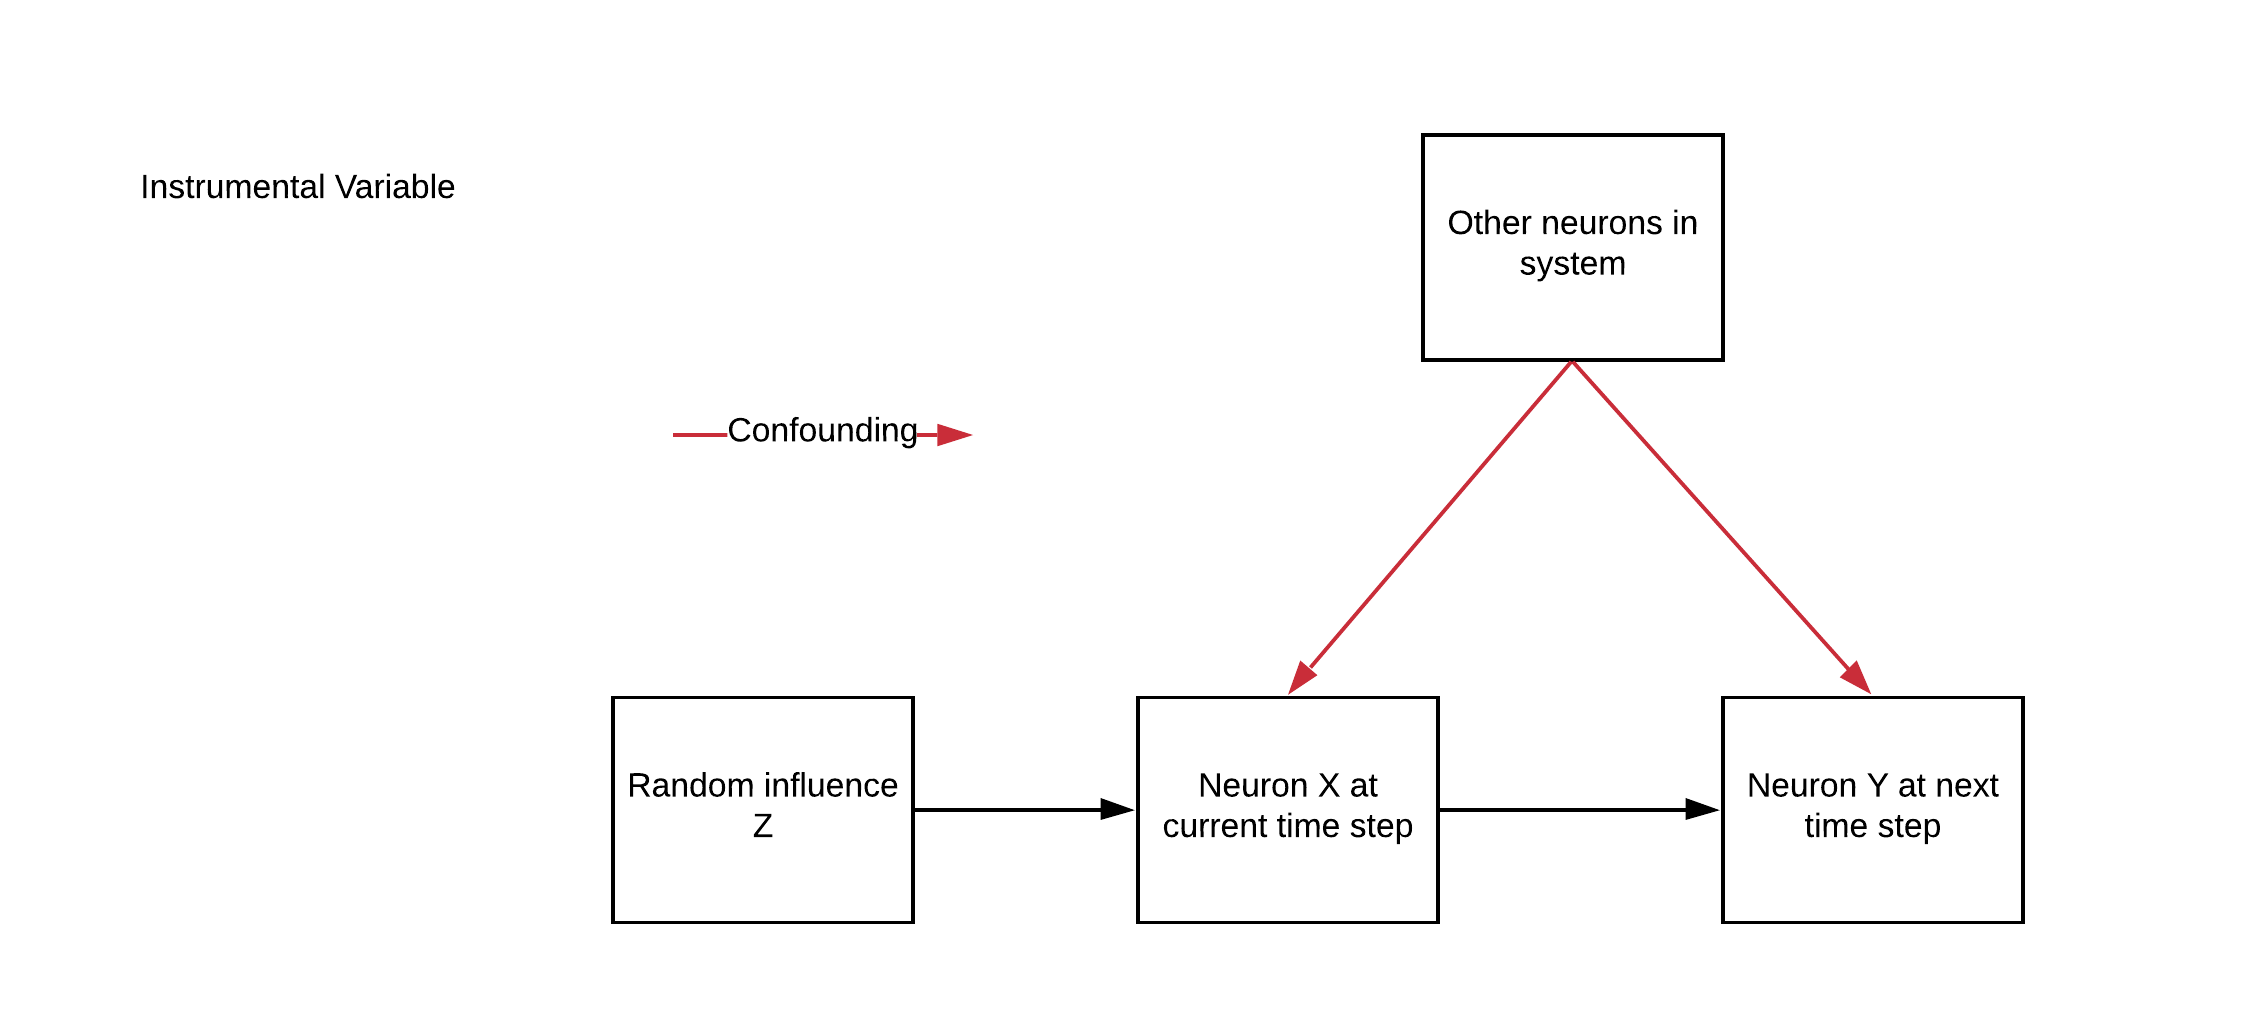
\includegraphics[scale=0.1]{Figures/NC/NC_Figure19.png}

\end{center}
\end{subbox}
\begin{subbox}{subbox}{  Simulate a system with IV
}
\scriptsize

\begin{center}
    
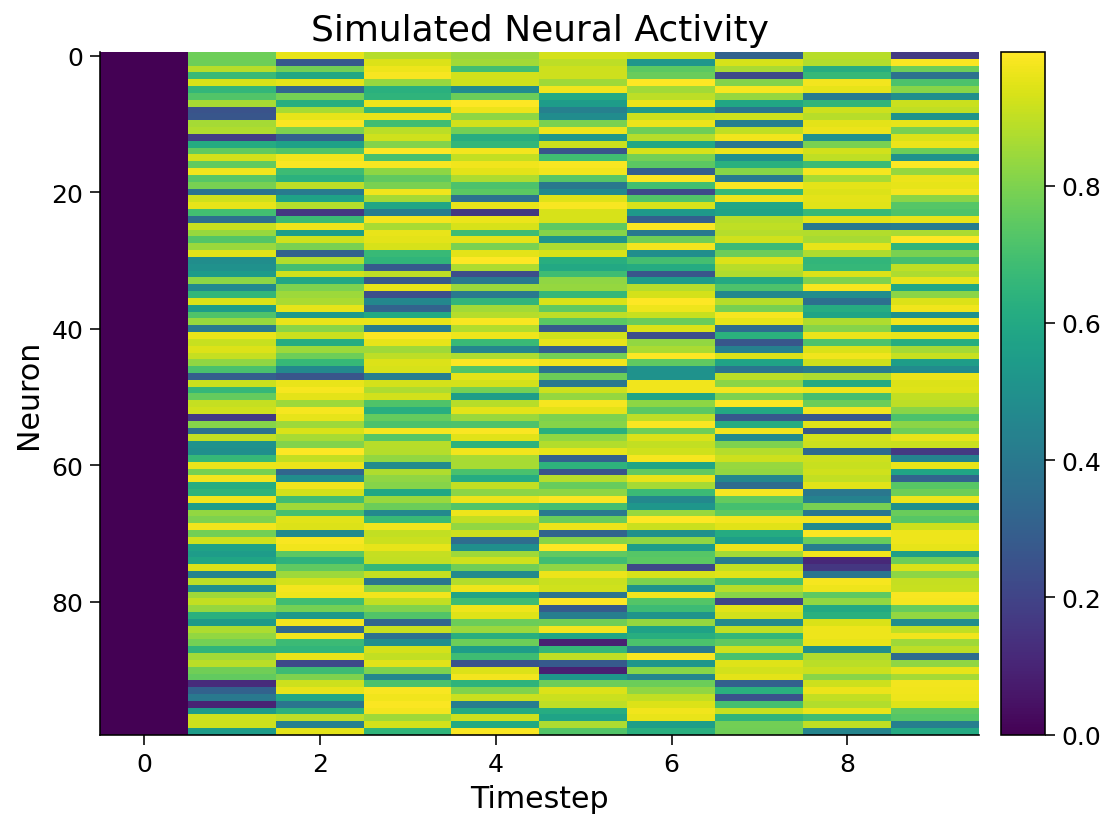
\includegraphics[scale=0.2]{Figures/NC/NC_Figure20.png}

\end{center}
\end{subbox}

\end{textbox}
%%%%%%%%%%%%%%%%%%%%%%%%%
%%%%%%%%%%%%%%%%%%%%%%%%%
\begin{textbox}{\href{https://compneuro.neuromatch.io/tutorials/W3D5_NetworkCausality/student/W3D5_Tutorial4.html}{Instrumental Variables (W3D5T4)}   }
\begin{subbox}{subbox}{ Estimate IV for simulated neural system
}
\scriptsize
Since you just implemented two-stage least squares, let's see how our IV estimates do in recovering the connectivity matrix.
\begin{center}
    
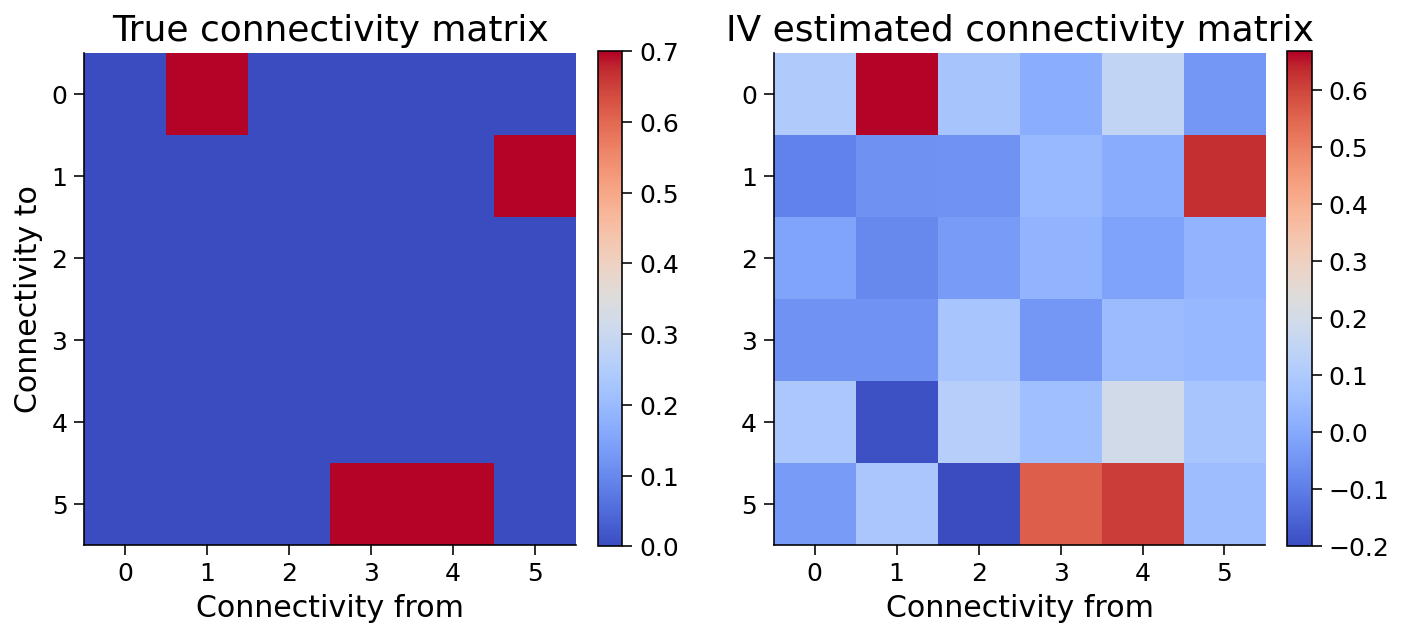
\includegraphics[scale=0.2]{Figures/NC/NC_Figure21.png}

\end{center}
The IV estimates seem to perform pretty well! In the next section, we will see how they behave in the face of omitted variable bias.

\end{subbox}

\begin{subbox}{subbox}{ IVs and omitted variable bias
}
\scriptsize
Changing the ratio of observed neurons and look at the impact on the quality of connectivity estimation using IV vs regression. The plots below are for a ratio of 0.6.

\begin{center}
    
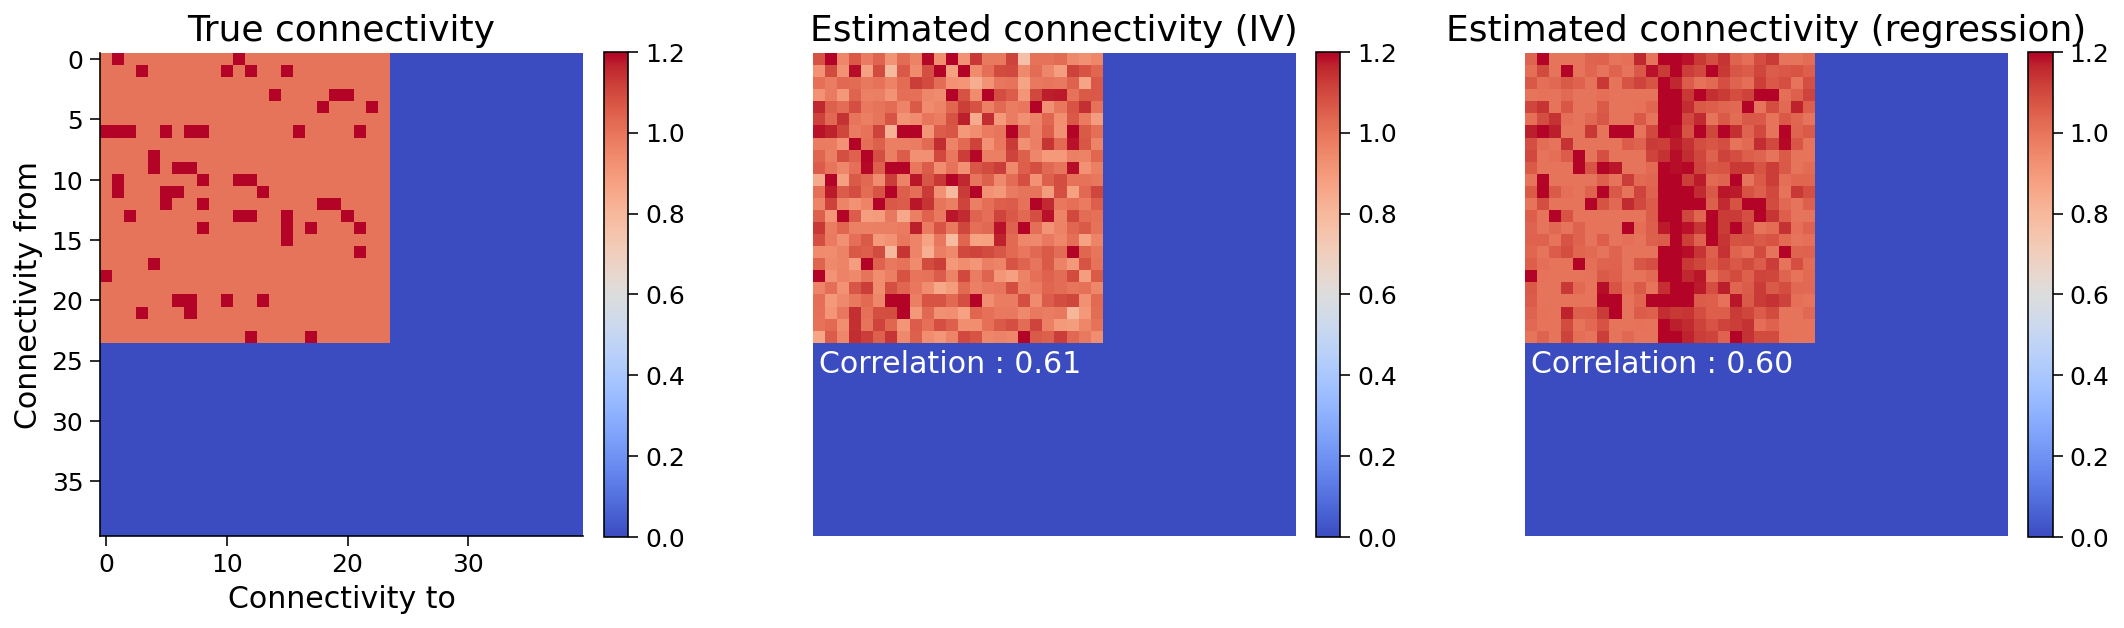
\includegraphics[scale=0.16]{Figures/NC/NC_Figure22.png}

\end{center}
We can also visualize the performance of regression and IV as a function of the observed neuron ratio below.

\begin{center}
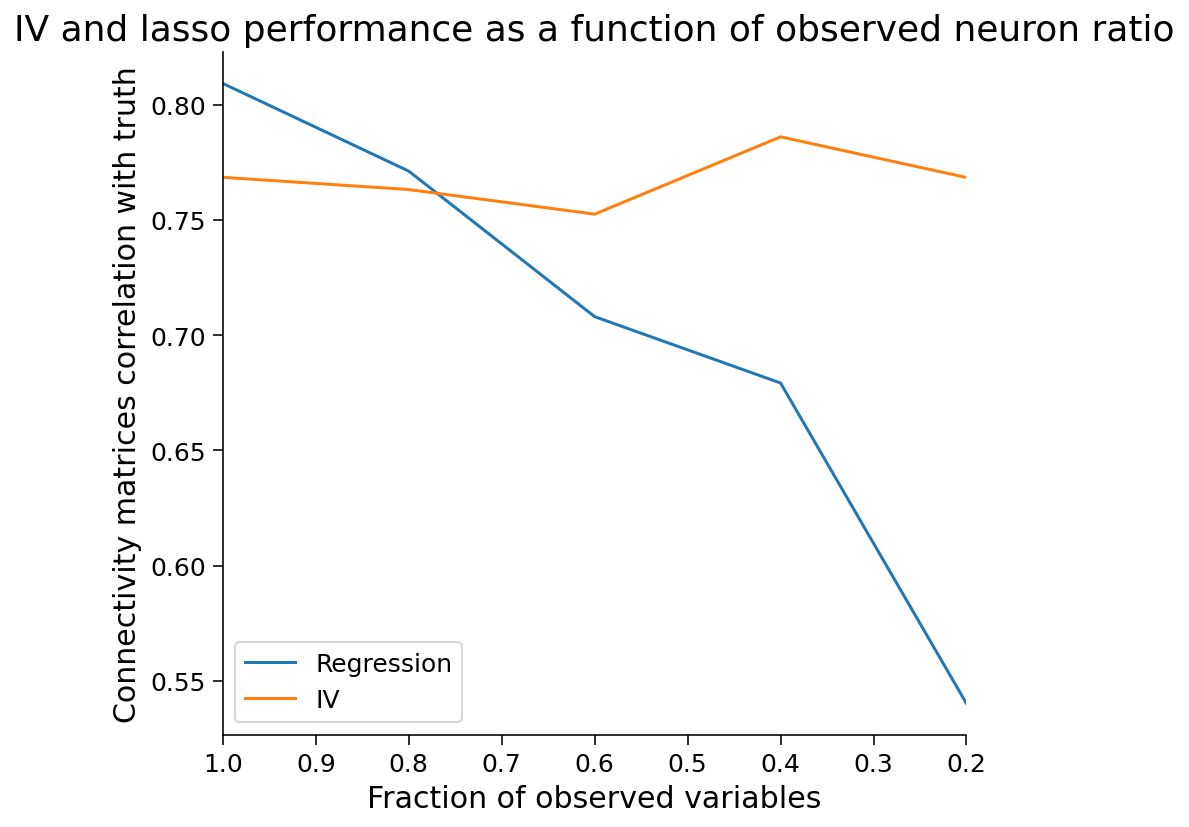
\includegraphics[scale=0.2]{Figures/NC/NC_Figure23.png}

\end{center}

We see that IVs handle omitted variable bias (when the instrument is strong and we have enough data).

\textbf{The costs of IV analysis}
\begin{itemize}
    

\item  we need to find an appropriate and valid instrument
\item  Because of the 2-stage estimation process, we need strong instruments or else our standard errors will be large
\end{itemize}
\end{subbox}
\end{textbox}
%%%%%%%%%%%%%%%%%%%%%%%%%
%%%%%%%%%%%%%%%%%%%%%%%%%